%%%%%%%%%%%%%%%%%%%%%%%%%%%%%%%%%%%%%%%%%%%%%%%%%%%%%%%%%%%%%%%%%%%%%%%%%%%%%%%
%
% Background
% 
%%%%%%%%%%%%%%%%%%%%%%%%%%%%%%%%%%%%%%%%%%%%%%%%%%%%%%%%%%%%%%%%%%%%%%%%%%%%%%%

\chapter{Theoretical background}
\label{sec:background}

\section{Fluid-Structure Interaction}
Fluid-Structure Interaction (FSI) studies the interaction between a structure (solid) and a fluid flow (liquid or gas) around it. It is a multi-physics problem which has large interest in diversified fields such as mechanical engineering (e.g. airfoils), civil engineering (e.g. towers) or medicine technique (e.g. artificial heart valves). Based on the response of structure and fluid fields, it is classified as one-way or two-way fluid-structure interaction problem. If the structural displacement/deformation does not influence the flow fluid or vice versa, then the FSI system is termed to be one-way fluid-structure interaction system. Conversely if the fluid flow and the displacement or deformation of the structure have significant influence on each other then the FSI system is termed as two-way fluid-structure interaction problem. Figure \ref{fig:2.1} represents a typical domain of a fluid-structure interaction problem, $\Omega$ refers to the common domain, $ \Omega_{f} $ the fluid domain and $ \Omega_{s} $ the structure domain. Figure   \ref{fig:2.2a} and \ref{fig:2.2b} represents one-way and two-way FSI fluid-structure interaction problems respectively.\\

\begin{figure}[H]
	\centering
	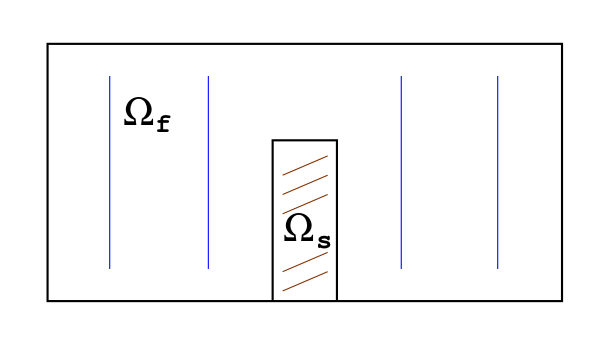
\includegraphics[height=3in]{fsi_domain}
	\caption{Representational figure of Fluid-Structure Interaction domain,taken from \citet{Richter}}
	\label{fig:2.1}
\end{figure}

\begin{figure}[h]
  \centering
  \captionsetup{justification=centering}
  \begin{subfigure}[b]{0.8\linewidth}
    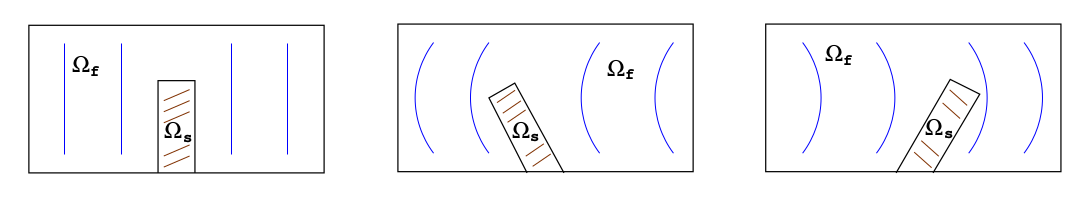
\includegraphics[width=\linewidth]{one-way-fsi}
    \caption{Structure domain influencing the fluid domain}
    \label{fig:2.2a}
  \end{subfigure}
  \begin{subfigure}[b]{0.8\linewidth}
    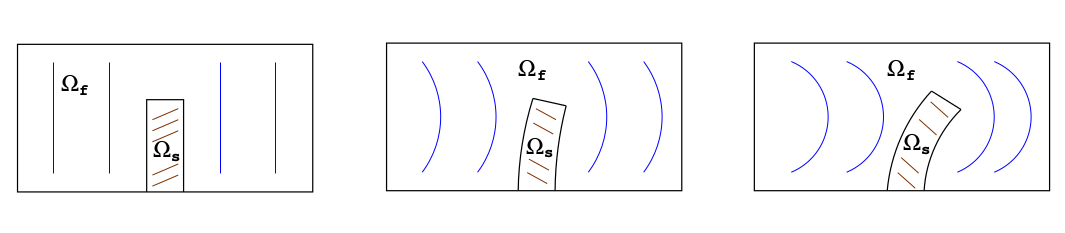
\includegraphics[width=\linewidth]{two-way-fsi}
    \caption{Both structure and fluid domains influencing each other}
    \label{fig:2.2b}
  \end{subfigure}
  \caption{Representational figure of one-way \ref{fig:2.2a}, and two-way \ref{fig:2.2b} fluid-structure interaction domains,taken from \citet{Richter}}
  \label{fig:2.2}
\end{figure}

\subsection{Numerical simulation strategies of FSI problems}
Numerical simulation of FSI involves solving set of differential equations and corresponding boundary conditions for fluid and structural fields respectively. Suitable interface conditions needs to be defined so as the structural and fluid domains are well distinguished. There are different methodologies implemented to solve the FSI problem and are well documented in the literature. An overview of the numerical solution procedure for FSI problems are presented below.\\
The FSI problem is classified based on solution approaches and on the treatment of mesh handling techniques as represented below. A brief overview of these methods are presented subsequently.

\begin{itemize}
 \item{Classification based on numerical solution approaches}
 \begin{itemize}
 \item{Monolithic solver}
 \item{Partitioned solver}
 \begin{itemize}
 \item{Explicit coupling}
 \item{Implicit coupling}
 \end{itemize}
 \end{itemize}
 \item{Classification based on meshing strategies}
 \begin{itemize}
 \item{Conforming mesh}
 \item{Non-conforming mesh}
 \end{itemize}
\end{itemize} 

\subsubsection{Classification based on numerical solution approaches}
This classification is based on how the fluid and structural fields are getting solved. In \textit{monolithic solvers} both the fluid and structural domains are expressed by single set of equations, whereas in \textit{partitioned solver approach} structural fields and fluid fields are solved separately and additionally requires coupling of the distinct solvers. A brief introduction to these methods are represented below.    

 \subsubsection*{Monolithic solver approach}
The equations governing the fluid flow and the displacement/deformation of the structure are represented by single set of equations which are then solved simultaneously by an unified algorithm, within a single solver framework \citet{{Richter},{Becker_2014},{hubner2004monolithic},{michler2004monolithic}}. The central idea of monolithic solvers is to represent the interface by an homogeneous discretization, thus maintaining the conservation properties at the interface \citet{michler2004monolithic} \citet{van2003energy}. Although monolithic approach gives strong coupling between the fields, it is commonly considered to be impractical for real world applications. It also demands enormous computational power for solving such a large system of equations since it has to incorporate the behavior of both fluid flow and solid structure. Figure \ref{fig:2.3} represents a schematic of the monolithic and partitioned solver approaches in solving FSI problems.
    	  
\begin{figure}[h]
  \centering
  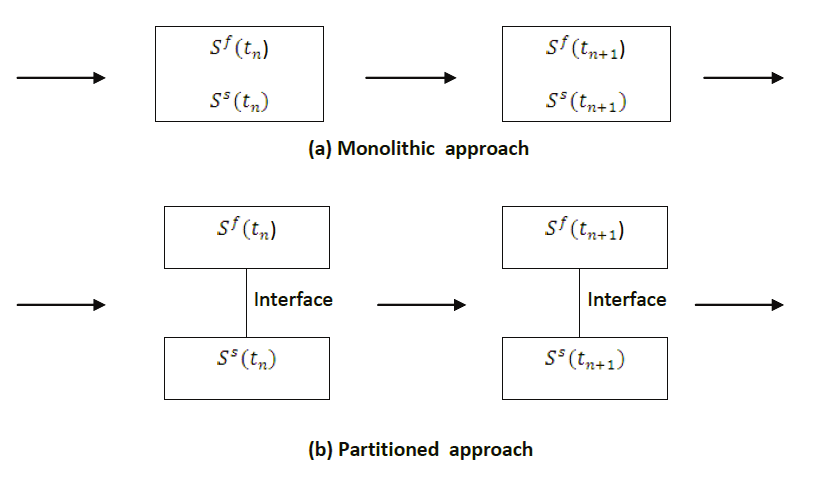
\includegraphics[width=1\linewidth]{monolithic}
  \caption{Schematic representation of Monolithic and Partitioned solution approaches. $ S^{f} $ represents the fluid solver and $ S^{s} $ represents the structural solver for two successive time steps current $ (t_{n}) $  and next $(t_{n+1})$. Figure taken from \citet{hou2012numerical}}
  \label{fig:2.3}
\end{figure}

 \subsubsection*{Partitioned solver approach}
Another approach to fluid-structure interaction is to use two distinct solvers to model both fluid and solid domains. This technique allows the coupling of the fluid and solid solution by maintaining suitable coupling conditions. The interfacial conditions are used explicitly to communicate information between the fluid and structure solutions.\\

Some coupling algorithms were suggested by various studies (\citet{{piperno1995partitioned},{felippa2001partitioned},{farhat2000two}}) which allows for reuse of existing codes that have been developed for each field. This approach is very robust and can be used for wide variety of applications. The major disadvantage of this approach is that, the interface location that divides the fluid and the structure domains is not known a priori and usually changes in time. Thus, the partitioned approach requires tracking of the new interface location and its related quantities, which can be cumbersome and error-prone. The interface coupling conditions that are as stated below, have to be satisfied in order to have a stable solution.

\begin{itemize}
\item Kinematic coupling condition: The displacements, velocities and accelerations of the sub-zones have to be equal at the interface at any point in time.

$\psi^{CFD}_{\Gamma}(t) = \psi^{CSD}_{\Gamma}(t)$, $\dot{\psi}^{CFD}_{\Gamma}(t) = \dot{\psi}^{CSD}_{\Gamma}(t)$, $ \ddot{\psi}^{CFD}_{\Gamma}(t) = \ddot{\psi}^{CSD}_{\Gamma}(t) $

\item Dynamic coupling condition: Conservation of the dynamic equilibrium of all forces at the interface needs to be satisfied. (Action and reaction forces must cancel out each other)

$ f^{CFD}_{\Gamma}(t) = -f^{CSD}_{\Gamma}(t) $
\end{itemize}

Depending on the influence of the structure movement on the fluid field the FSI problems are further subdivided into two following categories:

\begin{itemize}
 \item Explicit/Weakly coupled:	In an explicitly coupled algorithm, the equations of fluid mechanics,
structural mechanics and the relative mesh movement are solved sequentially. Initially the governing equation of fluid is solved with the velocity boundary condition derived from the structural displacement. The structural mechanics equations are solved next with the forces obtained from the fluid solver. Finally the grid is adapted based on the structural displacement. This coupling scheme is termed as weak coupling, as there is no sub iteration between the two sub zones.

 \item Implicit / Strongly coupled: In a strongly/implicitly coupled system, sub iterations between both the fluid and structural solvers are carried out at every time step till convergence is achieved.  The convergence is determined by maintaining a small enough structural residuum. Detailed explanation on this, is presented in the subsequent section. This approach is implicit in nature and more robust, however requires additional computation time.
\end{itemize}

Figure \ref{fig:2.4} represents the schematic representation of explicit and implicitly coupled, partitioned approach to solving fluid structure interaction. In the presented study \textit{semi-implicit predictor-corrector} coupling scheme is used. 

\begin{figure}[h]
  \centering
  \begin{subfigure}[b]{0.4\linewidth}
    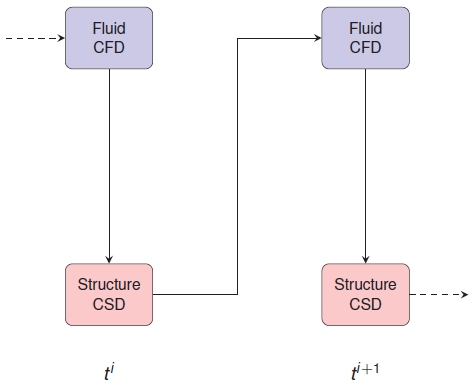
\includegraphics[width=2in]{explicit_coupling}
    \caption{Explicit coupling}
    \label{fig:2.4a}  
  \end{subfigure}
  \begin{subfigure}[b]{0.4\linewidth}
    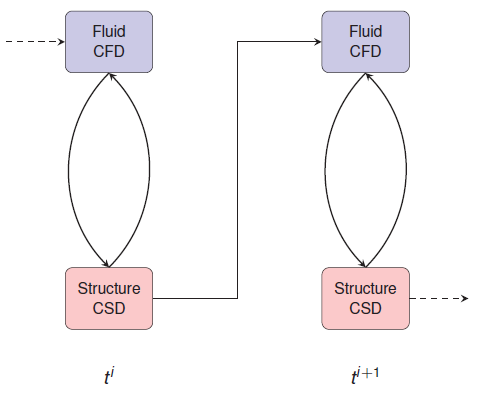
\includegraphics[width=2in]{implicit_coupling}
    \caption{Implicit coupling}
    \label{fig:2.4b} 
  \end{subfigure}
  \caption{Representational sketch of explicit coupling \ref{fig:2.4a}, and implicit coupling \ref{fig:2.4b} approaches to solving partitioned, fluid-structure interaction problems,taken from \citet{munsch2015entwicklung}}
  \label{fig:2.4}
\end{figure}

\subsection{Classification based on meshing strategies}\par
The FSI problem is further classified based on the meshing strategies implemented to couple the fluid and structure domains. They are classified into two methods:\textit{conforming mesh} and \textit{non-conforming mesh}\\

\begin{itemize}
 \item Conforming mesh method: In conforming mesh methods, the interface governing the fluid and structural domains is resolved such that the node connectivity is maintained between the domains. In this method, the interface conditions is considered as physical boundary conditions, which treat the interface location as part of the solution. Owing to the movement and/or deformation of the solid structure,re-meshing (or mesh-update) is required.
 
 \item Non-conforming mesh method: The non-conforming mesh methods treat the interface location as constraints imposed on the model equations so that non-conforming meshes (node-connectivity need not be maintained between the domains) can be employed. As a result, the fluid and solid equations can be conveniently solved independently from each other with their respective grids, and re-meshing is not necessary. The distinction between these two types of meshes can be observed in figure \ref{fig:2.5}, where a solid body (a sphere) is moving in a fluid domain.  
 \end{itemize} 
 
\begin{figure}[h]
  \centering
  \begin{subfigure}[b]{0.45\linewidth}
    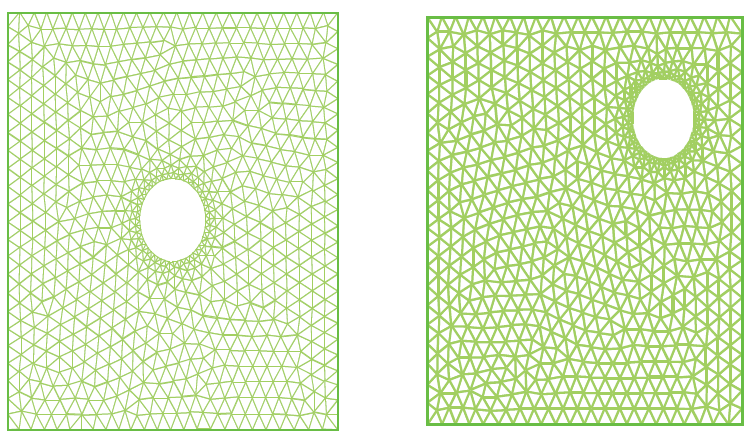
\includegraphics[width=2.25in]{conforming_mesh}
    \caption{Conforming mesh method representation at time $ t_{n} $ and $t_{n+1}$}
    \label{fig:2.5a} 
  \end{subfigure}
  \begin{subfigure}[b]{0.45\linewidth}
    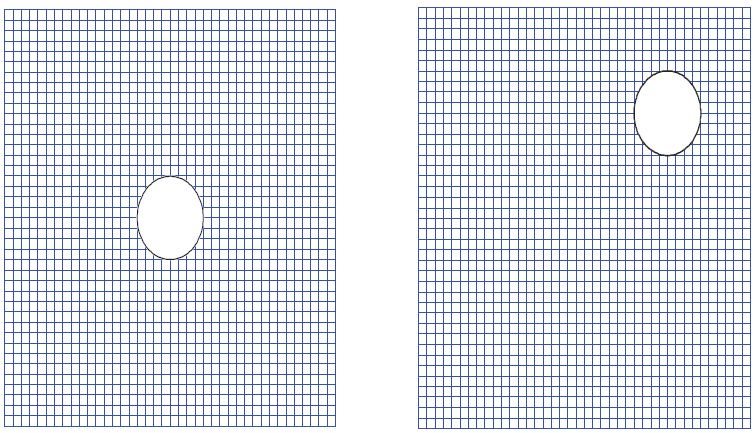
\includegraphics[width=2.25in]{non-conforming_mesh}
    \caption{Non-conforming mesh method representation at time $ t_{n} $ and $t_{n+1}$}
    \label{fig:2.5b}  
  \end{subfigure}
  \caption{Examples of Conforming mesh \ref{fig:2.5a} and Non-conforming mesh \ref{fig:2.5b} methods, taken from \citet{hou2012numerical}.}
  \label{fig:2.5}
\end{figure} 

\section{Governing equations of fluid flow and structural deformations}

In Fluid-Structure Interaction problems, the solid moves through the fluid domain due to different forces or excitation. The computation domain changes with time and must be considered during the simulation. An approach which aims to solve this particular problem is Arbitrary Eulerian Lagrangian formulation, popularly referred to ALE formulation. The governing equation for conservation of mass and momentum are reformulated for a moving grid which are time dependent control volume and surface integrals. The governing equations for a Newtonian incompressible fluid in ALE formulation is given as follows.

\begin{align}
%  {\frac{d}{dt}\int_{V(t)}\rho dV+\int_{S(t)}\rho(U-U_{g}).\vec{n} dS}=0 
 \frac{\partial{u_{j}}}{\partial{x_{i}}} & = 0\\
 \frac{\partial{u_{i}}}{\partial{t}}+\left(u_{i}-v_{g,i}\right)\frac{\partial{u_{i}}}{\partial{x_{j}}} &= \frac{1}{\rho}\frac{\partial{p}}{\partial{x_{i}}}+\nu\frac{\partial^2{u_{i}}}{\partial{x_{j}}\partial{x_{j}}}-\frac{\partial{\tau_{ij}}}{\partial{x_{j}}}\\
 \frac{1}{J}\frac{\partial{J}}{\partial{t}}-\frac{\partial{v_{g,i}}}{\partial{x_{i}}} & = 0
\end{align}\\
The equations presented are \textit{conservation of mass},\textit{conservation of momentum} and \textit{Space Conservation Law} (proposed by \citet{demirdvzic1988space}) in ALE formulation in order to account for the moving grid representation. Here $ v_{g} $ is the grid cell velocity and $J$ is the determinant of the metric tensor. Numerical treatment of these equations are presented in {refer to the relevant section}.

\subsection{Coupling of fluid and structural solvers}

The FSI problem in this study is solved by a \textit{semi-implicit predictor corrector} coupling scheme, which is a strong coupling method between fluid and structural solver. Details about this scheme is explained in \citet{breuer2012fluid}, summary of this scheme is presented in brief as follows:
\begin{enumerate}[(a)]
 \item At the start of the time step, the displacement of the structure is predicted based on values from the previous time step.
 \item A predictor corrector approach is implemented to solve for conservation of momentum and mass (velocity $u_{i}$ and pressure $p$). This is explained in detail in section {refer to relevant section}
 \item The calculated forces are then tranferred to the Computational Structural Dynamics (CSD) solver. Generalized-$\alpha$ method is used to solve the conservation equations of the structural solver. This is explained in detail in section {refer to relevant section}.
 \item The FSI-subiterations are performed until desired structural and fluid convergence is achieved for a particular time step. Dynamic calculation of the under-relaxation factor is used to enhance the convergence{refer to relevant section}. The corrector step takes the predicted velocity $\star{u}_{i}$ as approximation to obtain the new corrected velocity $u_{i}$ and pressure $p$. 
 \item Mesh adaptation for each FSI-subiteration is performed, based on transfinite interpolation by \citet{thompson1985numerical}. A comprehensive implementation can be found in \citet{munsch2011numerical}. 
\end{enumerate}
\par
The predcitor-corrector algorithm for a strongly coupled, partitioned FSI solver is represented in the flowchart \ref{fig:2.6}

\begin{figure}[h]
 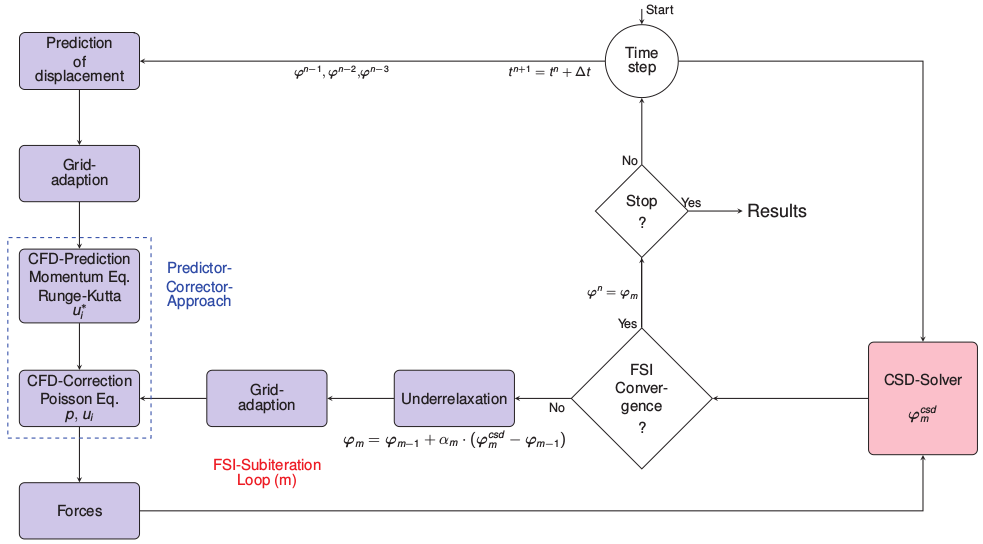
\includegraphics[height=3.5in]{p-c}
 \caption{Flowchart representing the predictor-corrector coupling scheme to solve a strongly coupled, partitioned FSI solver \citet{munsch2011numerical}}
 \label{fig:2.6}
\end{figure}

\subsubsection*{Convergence of the FSI sub-iterations}
As explained in flowchart \ref{fig:2.6} for an implicitly coupled, partitioned FSI solver, the flow field is determined in the actual flow geometry. From this, the friction and pressure forces on the
interacting walls are computed. These are boundary conditions to the structural solver. The structural solver computes the deformations, with which the fluid mesh is then modified. Afterwards the flow solver is started again. 

The FSI sub-iteration loop is repeated until a convergence criteria $\epsilon$ is satisfied, which is determined by the variation of the mean displacements \ref{eqn:2.4}.

\begin{equation}\label{eqn:2.4}
\frac{1}{N}\sum_{n=1}^{k}\frac{\norm{\mathbf{d}_{i-1}^{n}-\mathbf{d}_{i}^{n}}^2}{\norm{\mathbf{d}_{i}^{n}-\mathbf{d}_{i}^{n-1}}^2}<\epsilon
\end{equation}

In order to accelerate the rate of convergence, a relaxation factor is added to the displacement and force values. The resulting displacement is computed from the current sub-iteration displacement value and displacement value from the last sub-iteration. Under-relaxation of the displacements are done as given by the equation \ref{eqn:2.5}, where $\mathbf{\alpha}$ represents the under-relaxation factor.

\begin{equation}\label{eqn:2.5}
\mathbf{d}_{i}^{n}=\mathbf{d}_{i-1}^{n}+\mathbf{\alpha}\left(\tilde{\mathbf{d}}_{i}^{n}-\mathbf{d}_{i}^{n-1}\right)
\end{equation} 

Relaxation of the interface displacements is synonymous to the line search step of the non-linear solver. There are different methods to calculate the under-relaxation parameter. The most simplest method is by using a \textit{constant under-relaxation parameter} for all time-steps. There are various methods available now to determine the under-relaxation parameter dynamically, however the presented study focuses on \textit{Aitken relaxation method} and relaxation via the method of \textit{steepest descent}. An introduction to these methods is presented below.

\begin{enumerate}[(i)]
 \item Constant under-relaxation method: The most simplest and ineffective method is to choose a constant $\mathbf{\alpha}$ for all time-steps. The relaxation parameter has to be small enough to keep the iteration from diverging, but as large as possible in order to use as much of the new solution as possible and to avoid unnecessary FSI iterations. The optimal $\mathbf{\alpha}$ value is problem specific and not known a priori. Furthermore even the optimal fixed value could lead to more iterations than a suitable dynamic relaxation parameter.
 \item Aitken relaxation method: It is an effective and cheap method to calculate the under-relaxation parameter dynamically. The central idea of Aitken's $\bigtriangleup^2$ method is to use values from two previous iterations to improve the current solution, proposed by \citet{irons1969version}. The aitken factor $\mathbf{\mu}$ \ref{eqn:2.6} is calculated from the displacement values, and the under-relaxation factor $\mathbf{\alpha}$ is calculated as given in the equation \ref{eqn:2.9} \citet{mok2001partitioned}. This method has been implemented and validated with many FSI applications \citet{{kuttler2008fixed},{irons1969version}} .(Refer some more papers which uses aitken) The relaxation parameter calculation is valid in every FSI sub-iteration step. This method requires values from two previous sub-iterations, thus the relaxation parameter can be calculated after the first FSI sub-iteration. In the presented study the aitken factor from last time-step is used as an initial value for the current time-step $\left(\mathbf{\mu}_{i_{max}}^{n} = \mathbf{\mu}_{1}^{n+1}\right)$ as proposed by \citet{irons1969version}.      
\end{enumerate}
\begin{align}\label{eqn:2.6}
\mu_{i}^{n+1} &= \mu_{i-1}^{n+1}+\left(\mu_{i-1}^{n+1}-1\right)\frac{\left(\Delta\mathbf{d}_{i}^{n+1}-\Delta\mathbf{d}_{i+1}^{n+1}\right)^{T}\Delta\mathbf{d}_{i+1}^{n+1}}{\left(\Delta\mathbf{d}_{i}^{n+1}-\Delta\mathbf{d}_{i+1}^{n+1}\right)^{T}\left(\Delta\mathbf{d}_{i}^{n+1}-\Delta\mathbf{d}_{i+1}^{n+1}\right)}\\
\mathbf{d}_{i}^{n+1} &= \mathbf{d}_{i-1}^{n+1}-\mathbf{d}_{i}^{n+1}\\
\mathbf{d}_{i+1}^{n+1} &= \mathbf{d}_{i}^{n+1}-\tilde{\mathbf{d}}_{i+1}^{n+1}
\end{align}  
\begin{equation}\label{eqn:2.9}
\alpha_{i} = 1-\mu_{i}^{n+1}
\end{equation}
 
 












